
\documentclass[9pt,landscape]{extarticle}
\usepackage{amssymb,amsmath,amsthm,amsfonts}
\usepackage{multicol,multirow}
\usepackage{calc}
\usepackage{ifthen}
\usepackage[landscape]{geometry}
\usepackage[colorlinks=true,citecolor=blue,linkcolor=blue]{hyperref}
\usepackage{graphicx}
\usepackage{commath}
\usepackage{listings}
\usepackage{microtype}
\usepackage[compact,small]{titlesec}
\usepackage{enumitem}
\setenumerate{noitemsep,topsep=0pt,parsep=0pt,partopsep=0pt}
\setitemize{noitemsep,topsep=0pt,parsep=0pt,partopsep=0pt}
\graphicspath{ {./images/} }
\ifthenelse{\lengthtest { \paperwidth = 11in}}
    { \geometry{top=.5cm,left=.5cm,right=.5cm,bottom=.5cm} }
	{\ifthenelse{ \lengthtest{ \paperwidth = 297mm}}
		{\geometry{top=1cm,left=1cm,right=1cm,bottom=1cm} }
		{\geometry{top=1cm,left=1cm,right=1cm,bottom=1cm} }
	}
\pagestyle{empty}
\makeatletter
\renewcommand{\section}{\@startsection{section}{1}{0mm}%
                                {-1ex plus -.5ex minus -.2ex}%
                                {0.5ex plus .2ex}%x
                                {\normalfont\large\bfseries}}
\renewcommand{\subsection}{\@startsection{subsection}{2}{0mm}%
                                {-1ex plus -.5ex minus -.2ex}%
                                {0.3ex}%
                                {\normalfont\small\bfseries}}
\makeatother
\setcounter{secnumdepth}{0}
\setlength{\parindent}{0pt}
\setlength{\parskip}{0pt plus 0.5ex}
% -----------------------------------------------------------------------

\title{Cheat sheet}

\begin{document}

\raggedright
\footnotesize

\begin{center}
     \Large{\textbf{Computational Structure - Cheatsheet - W3-W5}} \\
\end{center}
\begin{multicols*}{5}
\setlength{\premulticols}{1pt}
\setlength{\postmulticols}{1pt}
\setlength{\multicolsep}{1pt}
\setlength{\columnsep}{2pt}


\section{Week 3}
\section{D-Latch}
Mux with a feedback loop
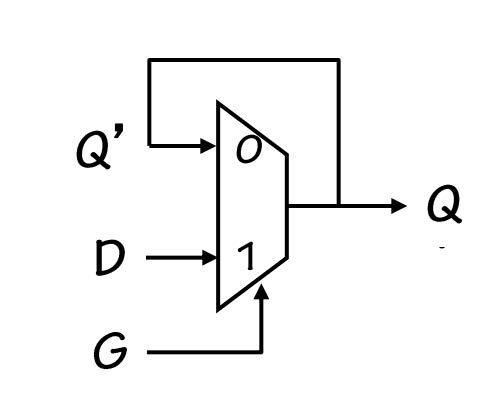
\includegraphics[width = 4.5cm]{D_latch}
-G represents the clock signal \\
-When G is 1, D is selected in the mux. (Write Mode) \\
-When G is 0,  Q follows Q'. (Read memory mode) \\
\subsection{Possible Problems}
Storing invalid information: If G changes from 1 to 0 at the exact momment when D is changing(invalid), the new invalid information of wire D will be stored instead \\
Unstable Output because of unstable input: In practice, input from users can be highly unstable. \\
\subsection{The Dynamic Discipline (addresses problem 1)}
The input to a synchronous sequential circuit must be stable
during the aperture (setup and hold) time around the clock
edge.
The dynamic discipline states that
\begin{enumerate}
\item $T_{setup} = 2t_{pd}$
\item $T_{hold} = t_{pd}$
\end{enumerate}
\begin{enumerate}
\item $T_{setup}$ = the minimum amount of time that the voltage on wire D needs to be stable before the clock edge changes from 0 to 1.
\item $T_{hold}$ = the minimum amount of time that the voltage on wire D needs to be stable after the clock edge changes from 0 to 1.
\item $t_{pd}$ is the propagation delay of the D-latch
\end{enumerate}
\section{Flip-Flop}
Created by putting 2 D-latches in series \\

\begin{enumerate}
\item There is an inverter on the G input on the master flip flop
\item When CLK signal is 0, the G wire of master latch receive a 1 while slave flip flop receive a 0 \\
Master latch : Write mode \\
Slave latch : Read memory mode
\item Vice-versa when CLk signal is 1
\item 1 D-Latch is on write mode why 1 D-latch is on memory mode at anytime.
\end{enumerate}
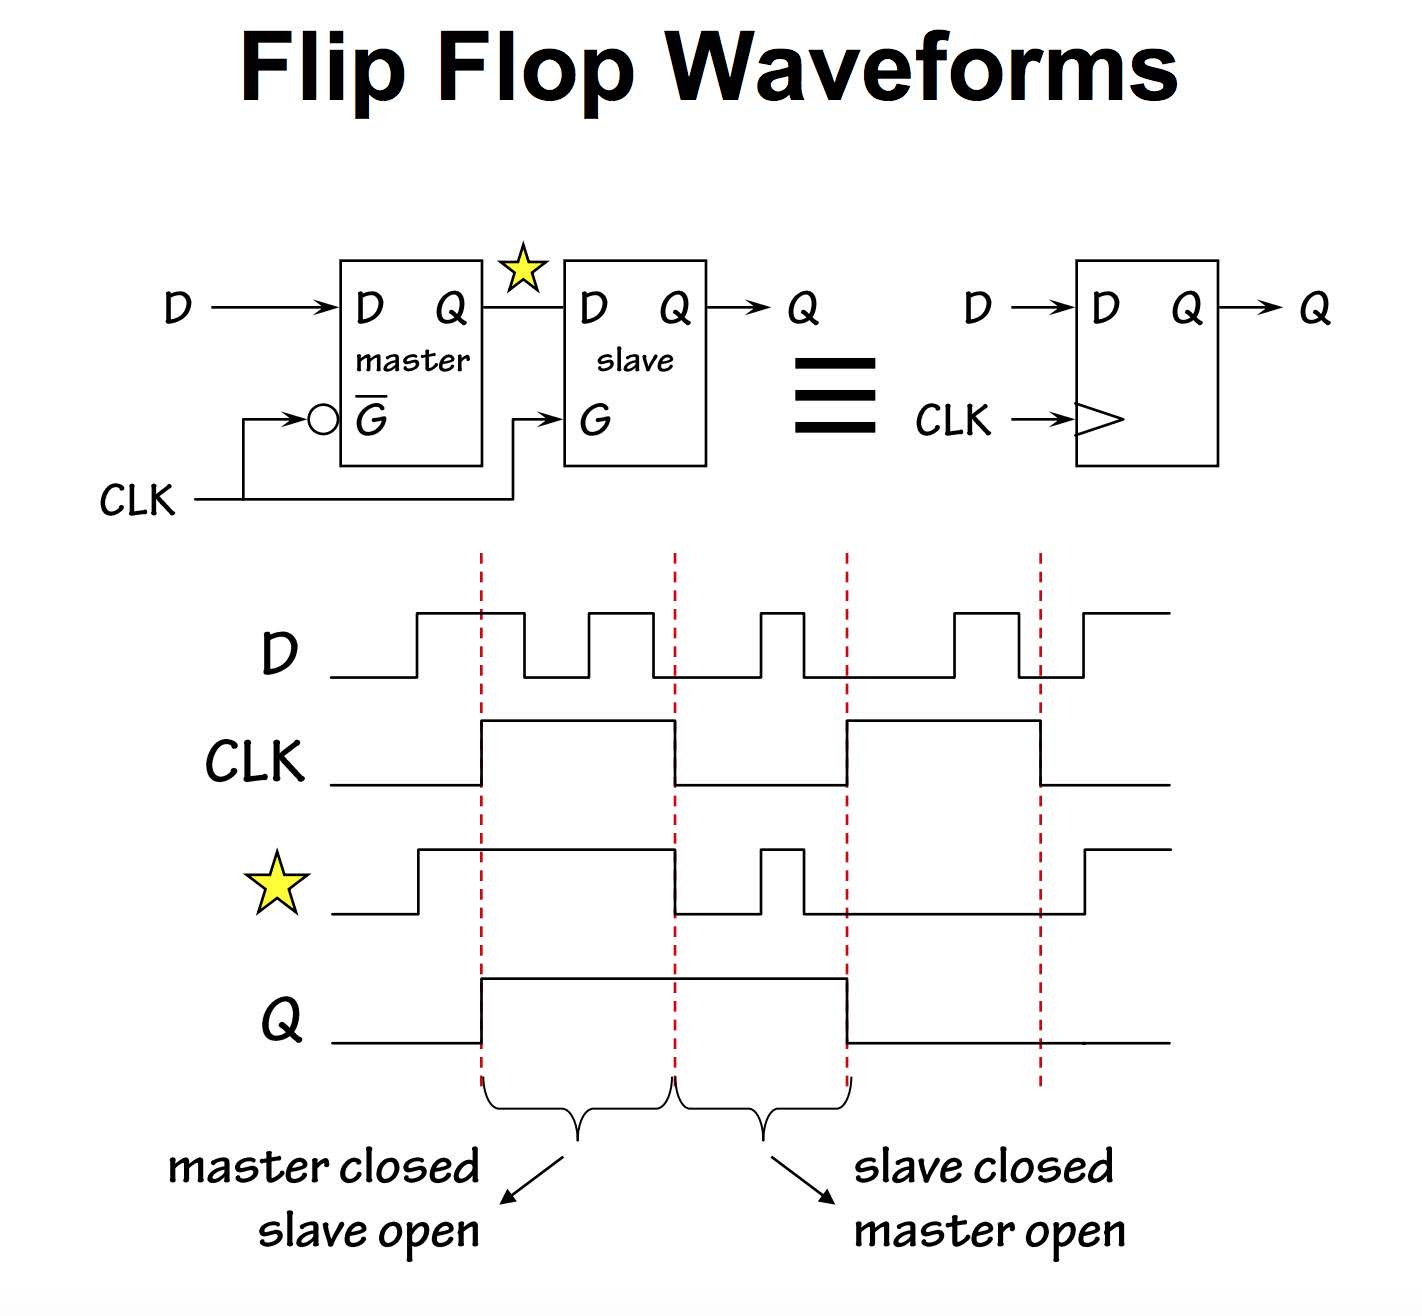
\includegraphics[width = 4.5cm]{Flip_flop_waveform}
Note that output wire Q only changes when CLK rises from 0 to 1
\subsubsection{Timing Constraint}
\begin{enumerate}
\item $t_{CD}$ of a D-latch is the time taken for invalid CLK input to produce an invalid output on wire G
\item $T_{PD}$ of a D-latch is the time taken for valid CLK input to produce a valid output on wire G
\end{enumerate}
\subsection{Flip-Flop Timing Constraint}
$t_{CD_{master}} > t_{HOLD_{slave}}$ \\
\begin{enumerate}
\item When signal at G in master changes from 1 to 0, and signal at G in slave
changes from 0 to 1, master goes into read memory mode and slave goes into
write mode.
\item Again, these CLK signals do not magically transform from 0 to 1 or 1 to 0. It
has to gradually change to high voltage ’1’ or to low voltage ’0’, and it will
crosses the invalid region (the region which voltage value doesn’t translate to
either digital 1 or 0).
\item Then $Q_{star}$ cannot change too quickly while G is transitioning, otherwise it will not
meet the hold time of the slave latch.
\item This means the contamination delay of the master latch has to meet the hold
time of the slave latch.
\end{enumerate}

\subsection{Sequential Logic Timing Constraint}
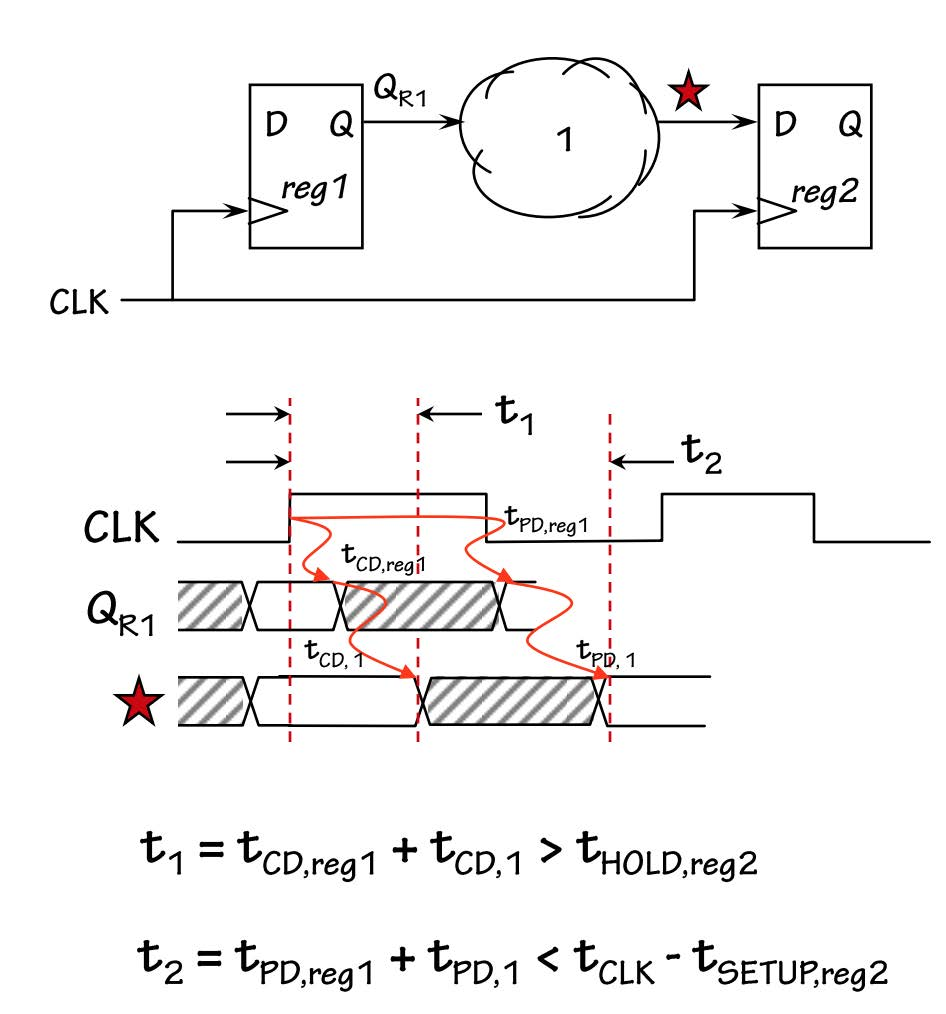
\includegraphics[width = 4.5cm]{Sequential_Logic} \\
$t_{work} = t_{PD}$


\section{Metastable State}
Properties
\begin{enumerate}
\item It corresponds to an invalid logic level
\item Unstable equilibrium which will settle to valid 0 or 1 eventually
\item Settling can be arbitraily long
\item All bistable system exhibits at least 1 metastable state
\item Cannot be avoided but can be minimize
\end{enumerate}

\subsubsection{Clock Skew}
$t_{1} = t_{CD,R1} + t_{CD,R1} > t_{HOLD,R2} + t_{skew}$ \\
$t_{2} = t_{PD,R1} + t_{PD,CL1} < t_{CLK} - t_{SETUP,R2} + t_{skew}$ \\





\section{Week 4}

\section{Programmable Machines}
\subsection{Programmable control system}
\begin{enumerate}
\item Control processing at each step with FSM
\item Allow different control sequences to be loaded into control FSM
\item Re-use data path and reconfigure FSM to compute new function
\end{enumerate}
\subsection{Short-comings}
\begin{enumerate}
\item Tiny repertoire of operation
\item Unable to generate and execute a new program
\item Limited storage
\end{enumerate}
\subsection{Finate State Machine: Enumeration}
FSM with \textit{i} inputs, \textit{o} outputs, \textit{s} states 
\begin{enumerate}
\item Truth table has $2^{i + s}$ rows with (o + s) columns each
\item $2^{(o + s) 2^{i + s}}$ max state
\item Limitation : cannot solve problems with arbitrarily many states
\end{enumerate}

\subsection{Turing Machines}
Turing Machine Specification
\begin{enumerate}
\item Doubly-infinite tape
\item Discrete symbol positions
\item Finite alphabet
\item Control FSM \\
Inputs - Current Symbol \\
Outputs - Write 0/1 , move Left/Right 
\item Initial Starting State {S0}
\item Halt State{Halt}
\end{enumerate}
Properties
\begin{enumerate}
\item Can be used to compute integer functions of form $y = T_{k}[x]$ 
\item Where k: FSM index, x: input tape configuration, y: output tape configuration. \\
*Not all integer functions can be computed with Turing Machines
\item Computable functions : f(x) computable $\Leftrightarrow \exists k : \forall x: f(x) = T_{k}[x] = f_{k}(x)$
\item Church-Turing Hypothesis states that any computable function is computable by a TM
\end{enumerate}

\subsection{Universal Functions and Universality}
Universal function: $U(k,j) = T_{k}(j)$ \\
U is comptable by a Turing Machine \\
$\rightarrow$ k encodes a 'program' \\
$\rightarrow$ j encodes the input data to be used \\
$\rightarrow T_{u}$ interprets program



\section{Von Neumann Model}
4 components
\begin{enumerate}
\item CPU - contains several registers as well as logic
\item Memory = storage of N words with W bits, where W is a fixed architerctural paramter, and N can be expanded to meet needs
\item Input/Output 
\item Connection Bus
\end{enumerate}


\section{Week 5}
\section{Machine Language and Compilers}
\subsection{Compiler}
\begin{enumerate}
\item Complier translate high-level language into low-level assembler machine language
\item Done before execution and slows program development
\item Decisions made during compile time,before execution
\end{enumerate}
\subsection{Interpreter}
\begin{enumerate}
\item Computes exact instructinos
\item Done after execution and slows down program execution
\item Decisions made during run time, after execution
\end{enumerate}
\section{UASM}
\begin{enumerate}
\item LONG tells the assembler to assemble a 32 bit quantity
\end{enumerate}


\section{Stacks and Procedures}
\begin{enumerate}
\item Add one item at a time to the top of the stack by PUSH, and remove one item at a time from the top of the stack by POP
\item Stack pointer (SP) points to the available memory location to write to (first unused stack space). SP is actually the content of R29.
\item base pointer (BP) points to the base of the stack, or equivalently first item pushed to the stack.
\item There are only 2 operations to modify a stack: Push and Pop
\item In the ’original state’ of the diagram, the SP is set to address 0x0000 1000
\item Push is a 2 step procedure: \\
- Increase value of SP by 4 byte \\
- Writing data to SP - 4
\item Pop is also a 2 step procedure: \\
- store data at addressed pointed by SP \\
- reduce value of SP by 4 byte
\end{enumerate}


\section{Some Beta Documentation}
\begin{itemize}
\item BEQ/BF - If Ra = zero, the PC is loaded with the target address; \\
literal = ((OFFSET(label) - OFFSET(current instruction)) / 4) - 1 \\
PC $\leftarrow$ PC + 4 \\
EA $\leftarrow$ PC + 4*SEXT(literal) \\
TEMP $\leftarrow$ Reg[Ra] \\
Reg[Rc] $\leftarrow$ PC \\
if TEMP = 0 then PC $\leftarrow$ EA \\
\item JMP - \\
PC $\leftarrow$ PC+4 \\
EA $\leftarrow$ Reg[Ra] and 0xFFFFFFFC \\
Reg[Rc] $\leftarrow$ PC \\
PC $\leftarrow$ EA \\

\item LDR - The effective address EA is computed by multiplying the sign-extended literal by 4 (to
convert it to a byte offset) and adding it to the updated PC. The location in memory specified
by EA is read into register Rc. The Ra field is ignored and should be 11111 (R31). The
supervisor bit (bit 31 of the PC) is ignored (i.e., treated as zero) when computing EA. \\
literal = ((OFFSET(label) - OFFSET(current instruction)) / 4) -1 \\
PC $\leftarrow$ PC + 4 \\
EA $\leftarrow$ PC + 4*SEXT(literal) \\
Reg[Rc] $\leftarrow$ Mem[EA] \\

\item Stack pointer (SP) points to the available memory location to write to (first unused stack space). SP is actually the content of R29.

\end{itemize}

\section{Finding Setup Time for Input}
\begin{enumerate}
\item CASE 1: INPUT --> REGISTER \\
$t_{S} = t_{S_{R1}}$
\item CASE 2: INPUT --> CL --> REGISTER \\
$t_{S} = t_{pd_{CL1}}+ t_{S_{R1}}$
\end{enumerate}

\section{Finding Hold Time for Input}
\begin{enumerate}
\item CASE 1: INPUT --> REGISTER \\
$t_{H} = t_{H_{R1}}$
\item CASE 2: INPUT --> CL --> REGISTER \\
$t_{H} = t_{H_{R1}}+ t_{cd_{CL1}}$
\end{enumerate}

\section{Propagation and contamination delay of  circuit}
Propagation delay : The time taken to produce a valid output after the CLK rise turns valid \\
Contamination delay : The time taken to produce an invalid output after the CLK turns invalid \\
\begin{enumerate}
\item CASE 1: REGISTER --> OUTPUT\\
$t_{cd} = t_{cd_{R1}}$
\item CASE 2: REGISTER --> CL --> OUTPUT \\
$t_{pd} = t_{pd_{R1}}+ t_{pd_{CL1}}$ \\
$t_{cd} = t_{cd_{R1}}+ t_{cd_{CL1}}$
\end{enumerate}

\end{multicols*}
\begin{multicols*}{4}



\section{Finding the minimum CLK period}
According to timing constraint t2, the clock period has to be larger than the time
taken to finish the ’work’ (propagation delays plus the setup time of the downstream
register) between two registers. (Diagram on back-end)

\begin{enumerate}
\item At each clock period (each time the clock rise from 0 to 1), a new input is being
”loaded” to the registers, and the previous input is passed through to the rest
of the components downstream
\item So before the next clock rise, one has to finish all the necessary work downstream
until the next register, in this case the next register is R2.
\item There are two paths, blue and red where the output of R1 will flow downstreams.
\item The time taken for the blue path to ’work’ (propagation delays plus setup time
for the first register downstream blue path) is: \\
$t_{blue} = t_{pd_{R1}}+ t_{pd_{CL1}} + t_{pd_{CL3}} + t_{S_{R3}}$ \\
\item The time taken for the red path to ’work’ (propagation delays plus setup time
for the first register downstream red path) is: \\
$t_{red} = t_{pd_{R1}}+ t_{pd_{CL2}} + t_{S_{R2}}$ \\
\item Both blue path and red path ’work’ has to be done before the next clock rise 
\item Hence minimum CLK period is max of $t_{blue} , t_{red}$

\end{enumerate}


\section{Writing Assembly Language Procedure}
\begin{enumerate}
\item Calling Sequence - Arguments - (Write) push arguments into the stack in the reverse order. \\ 
write a constant into the register using CMOVE, and then push it into the memory.
\item Calling Sequence - Branching and Cleanup - (Write) - call the function itself using
BR , and then write cleanup codes (Deallocate).
\item Standard Entry Sequence \\
PUSH(LP) \\
PUSH(BP) \\
MOVE(SP,BP) \\
\item The Actual Code
\item Exit Sequence - Pop Regs from Actual Code
\item Exit Sequence - Standard Exit Sequence \\
MOVE(BP,SP) \\
POP(BP) \\
POP(LP) \\
JMP(LP) \\
\end{enumerate}






\setlength{\premulticols}{1pt}
\setlength{\postmulticols}{1pt}
\setlength{\multicolsep}{1pt}
\setlength{\columnsep}{2pt}
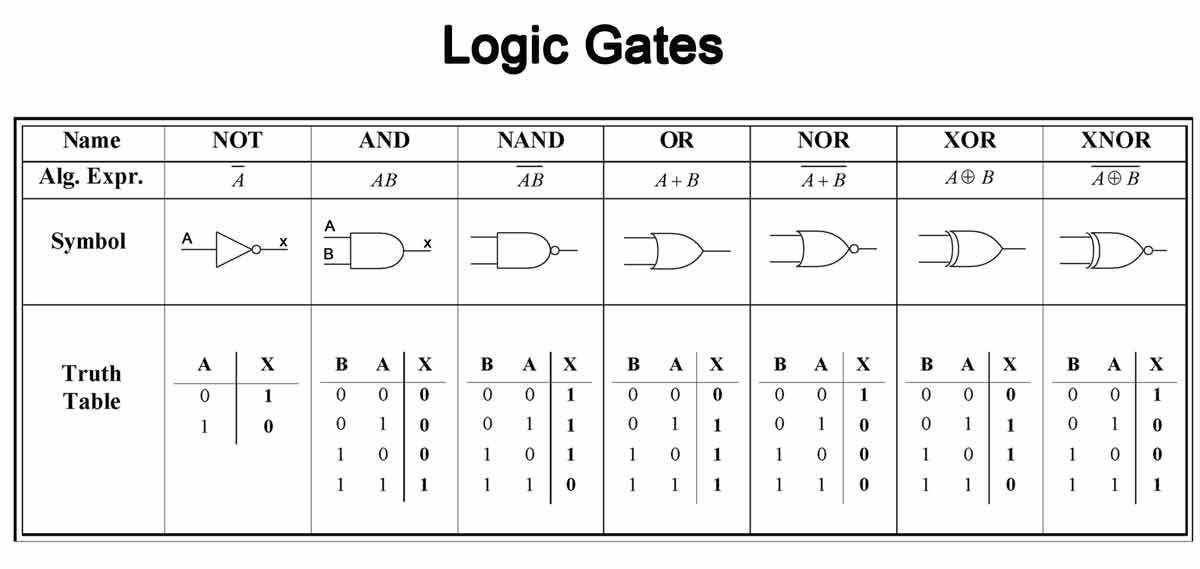
\includegraphics[width = 7cm]{Logic_gates}
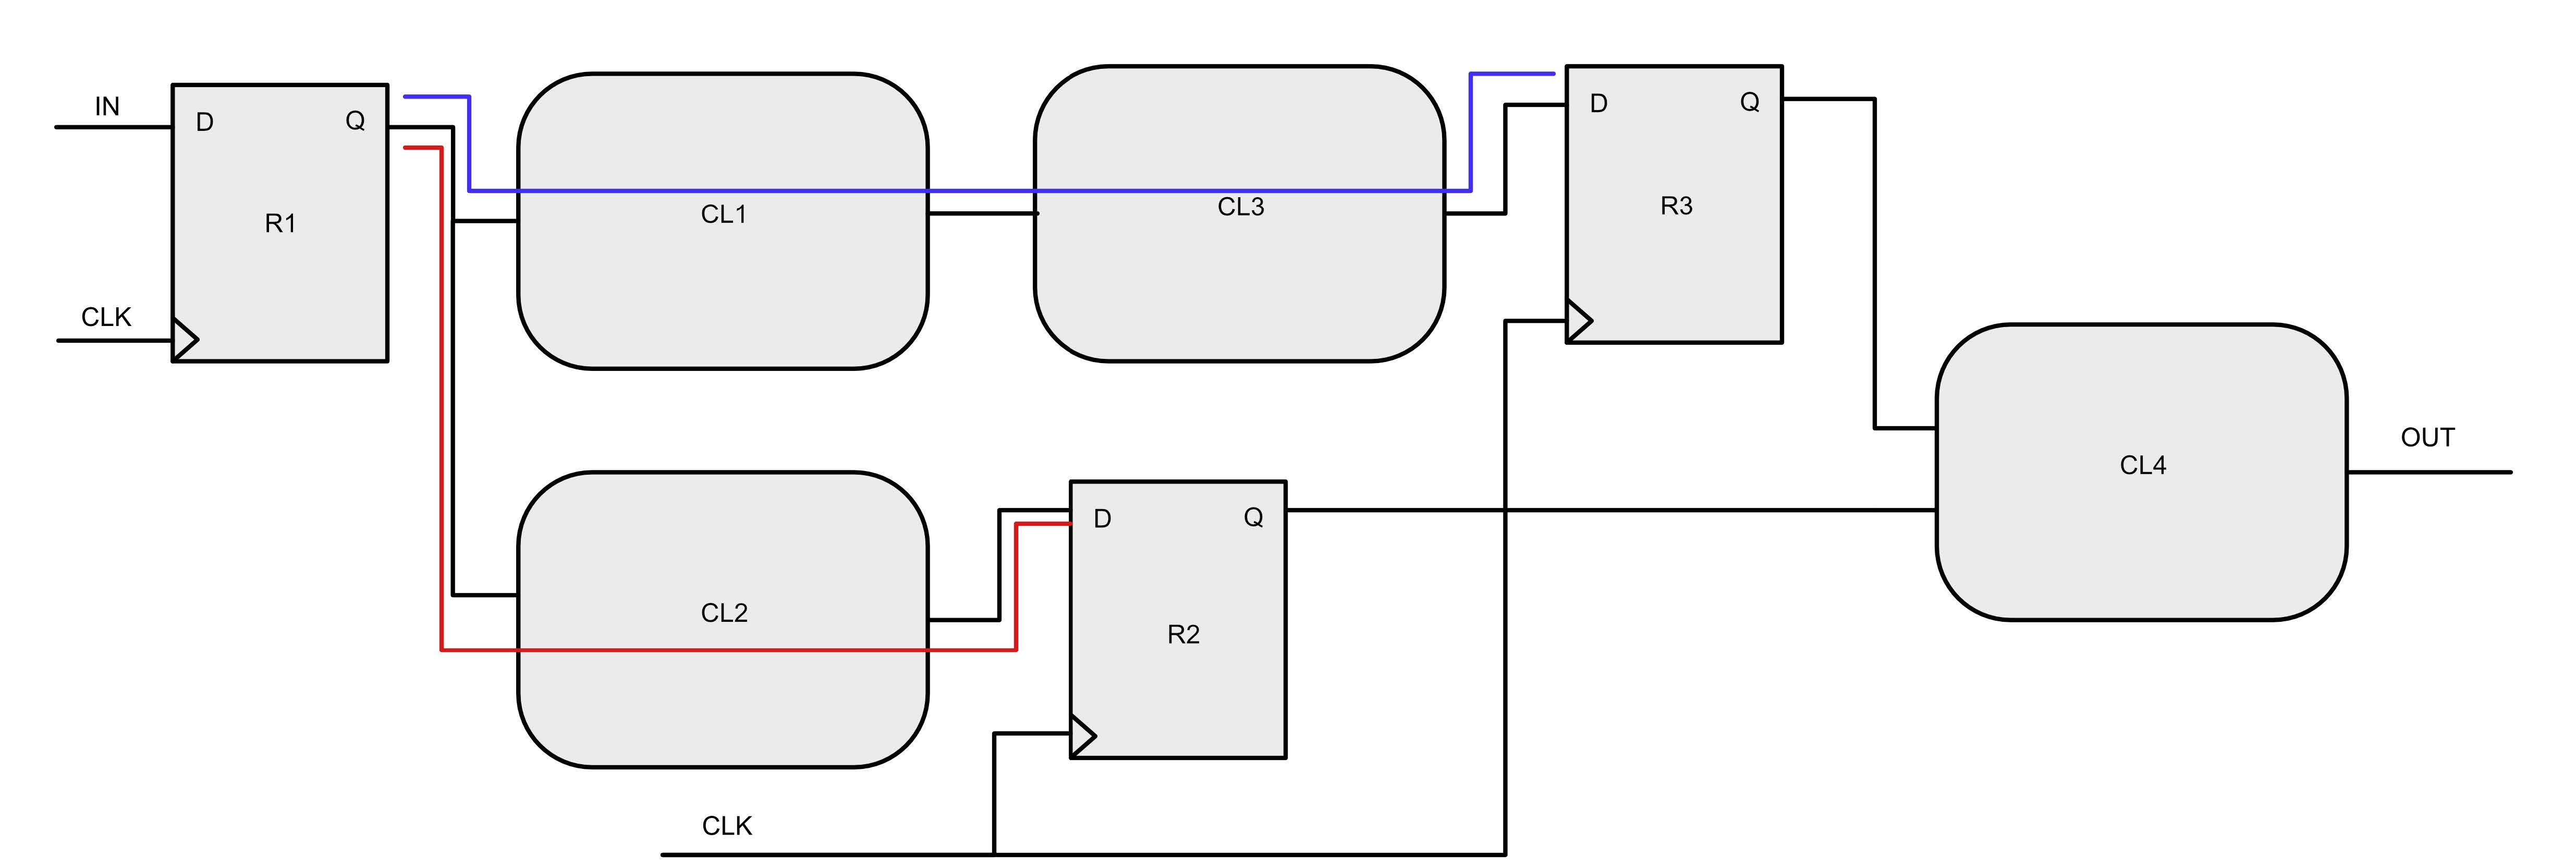
\includegraphics[width = 7cm]{CLK}
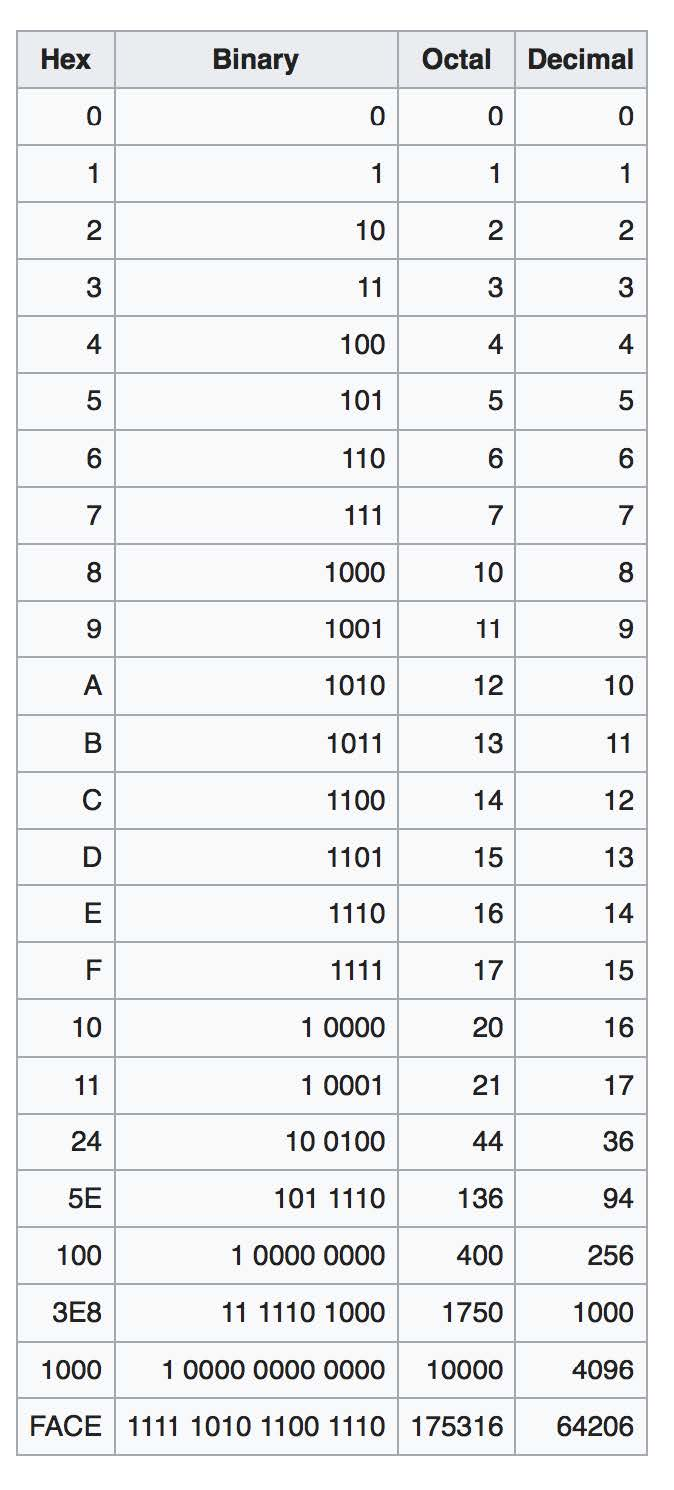
\includegraphics[width = 5cm]{Conversion_table}

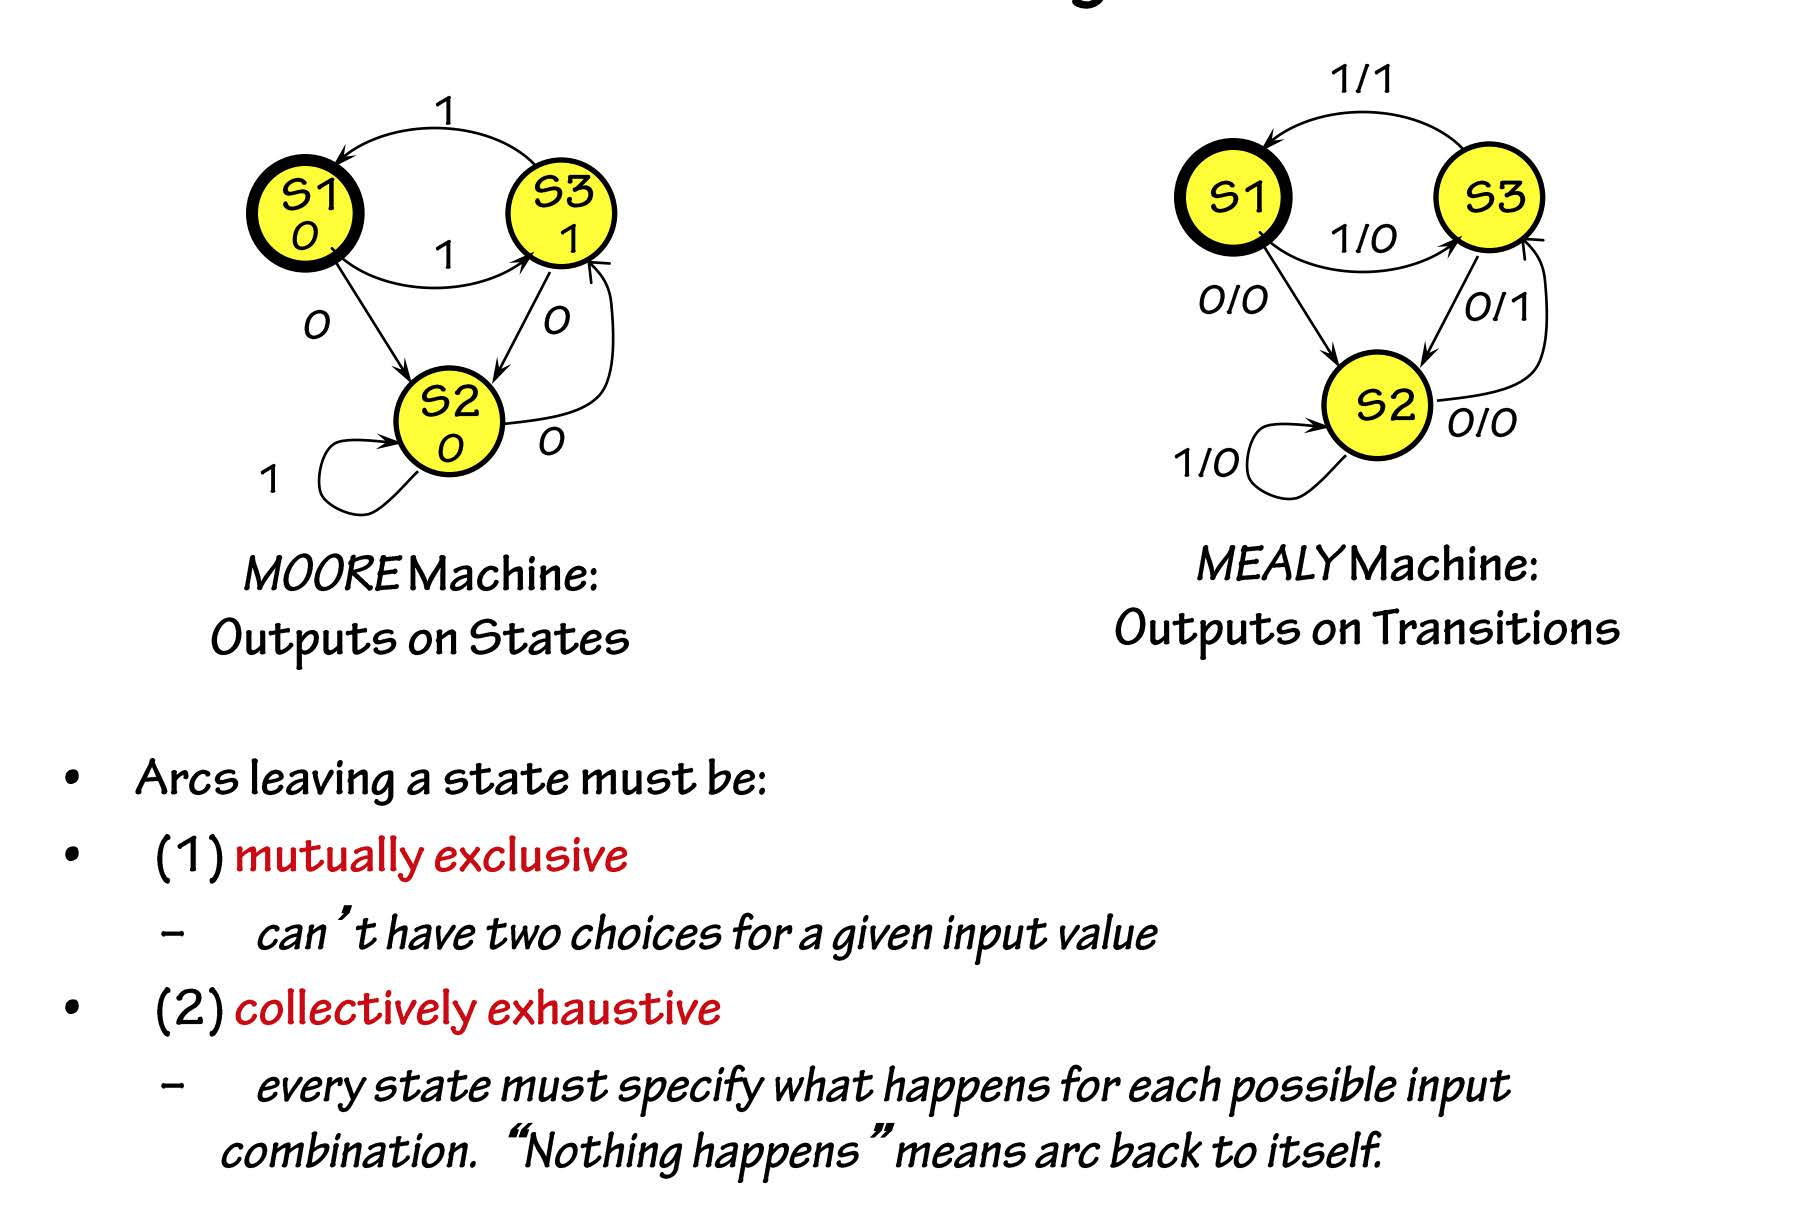
\includegraphics[width = 7cm]{State_machine}
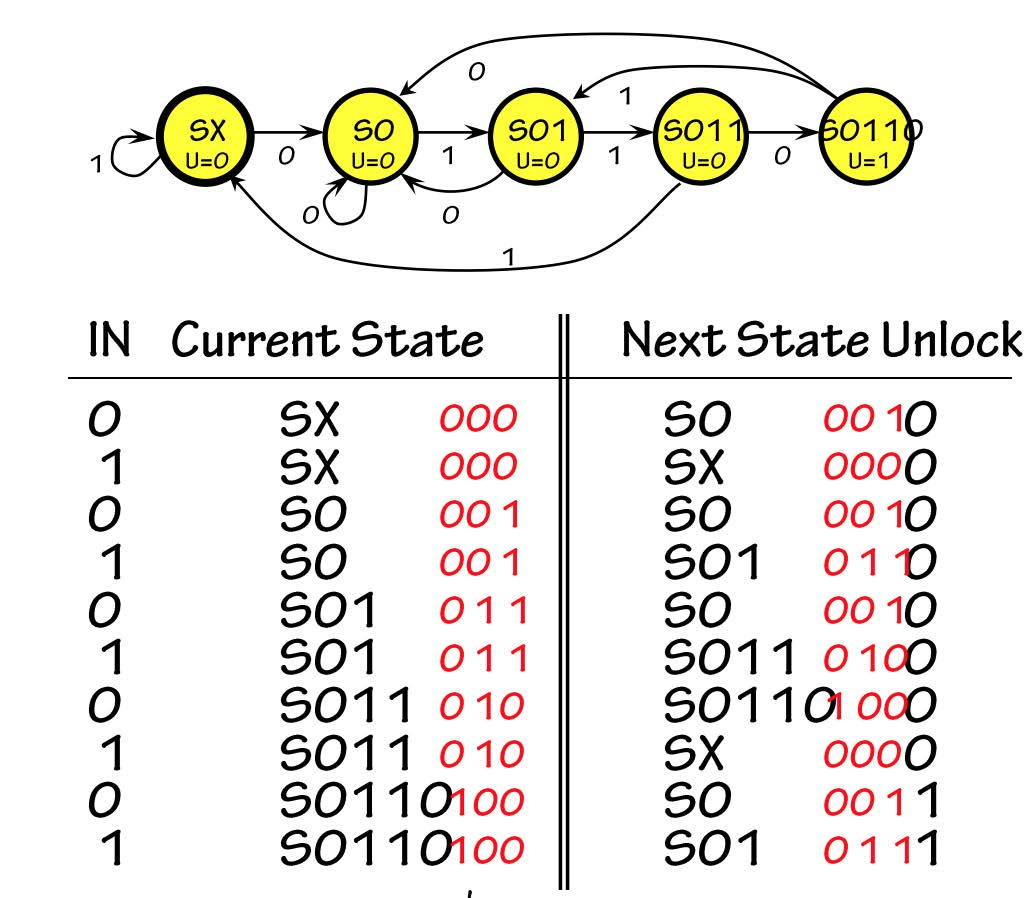
\includegraphics[width = 5cm]{state_transition}
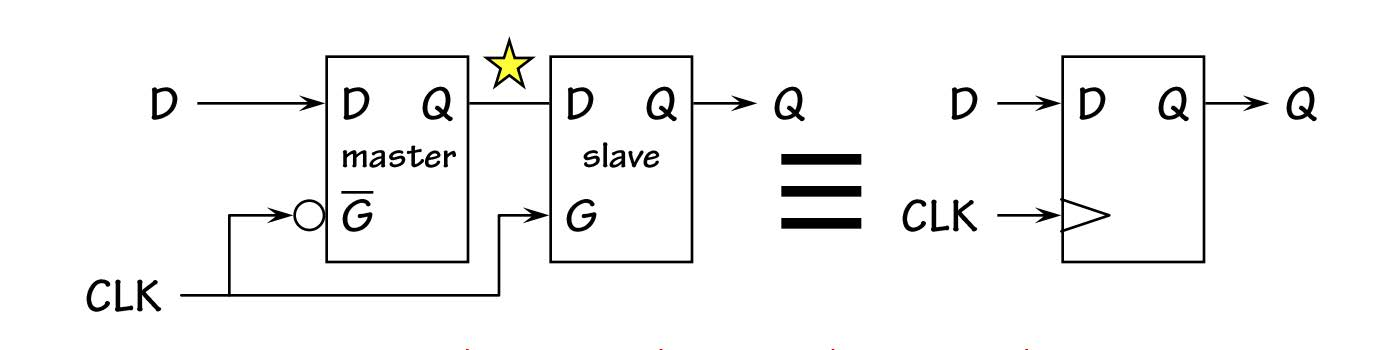
\includegraphics[width = 7cm]{Flip_flop_Diagram}

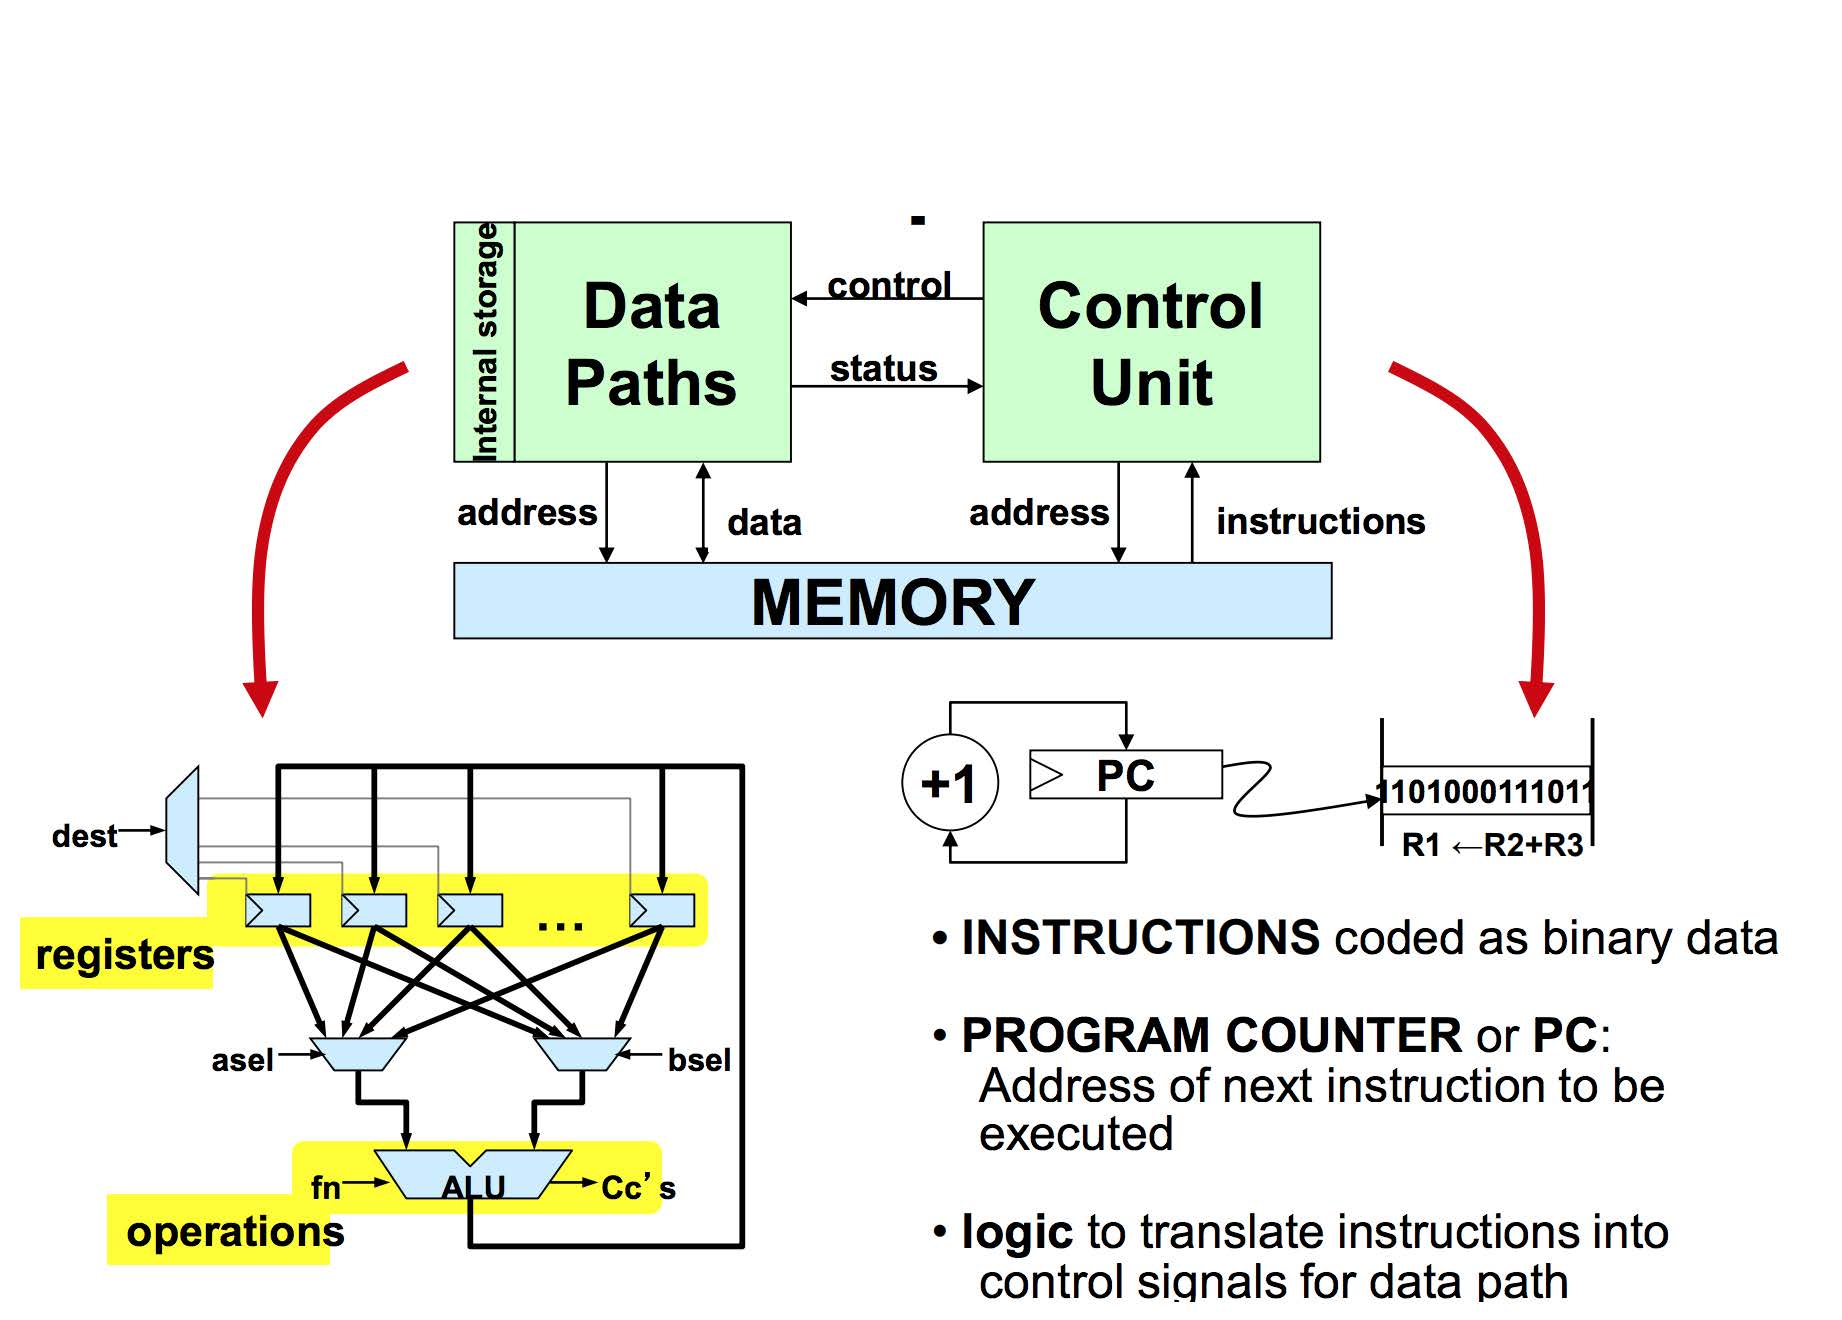
\includegraphics[width = 7cm]{CPU_anatomy}

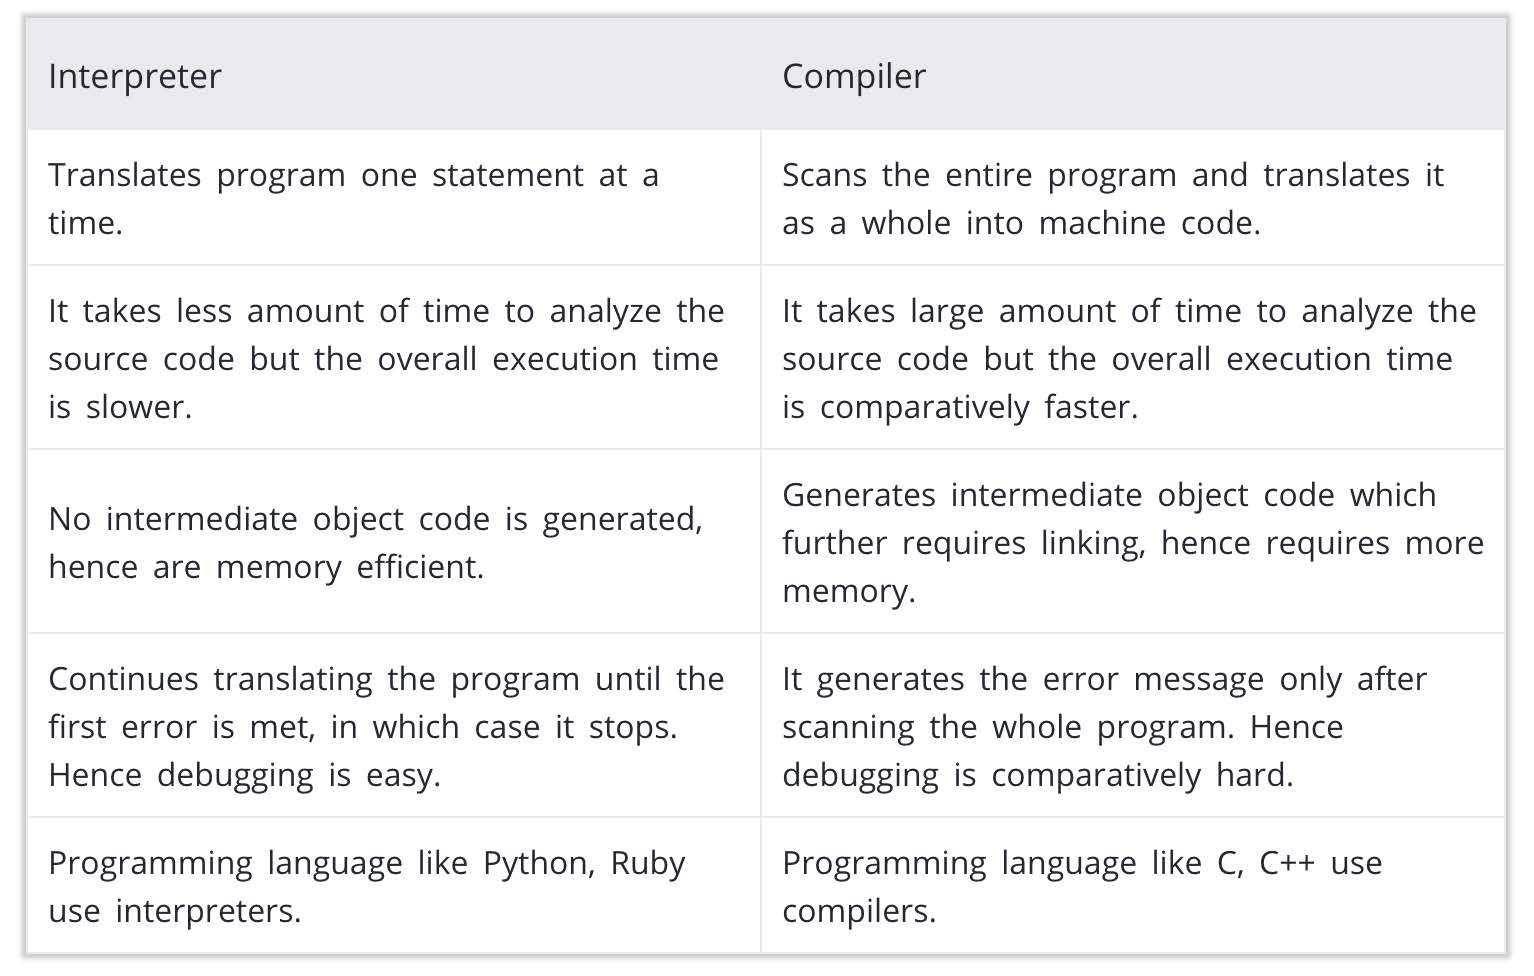
\includegraphics[width = 7cm]{Interpreter_Compiler}
\includegraphics[width = 12cm]{Stackframe}
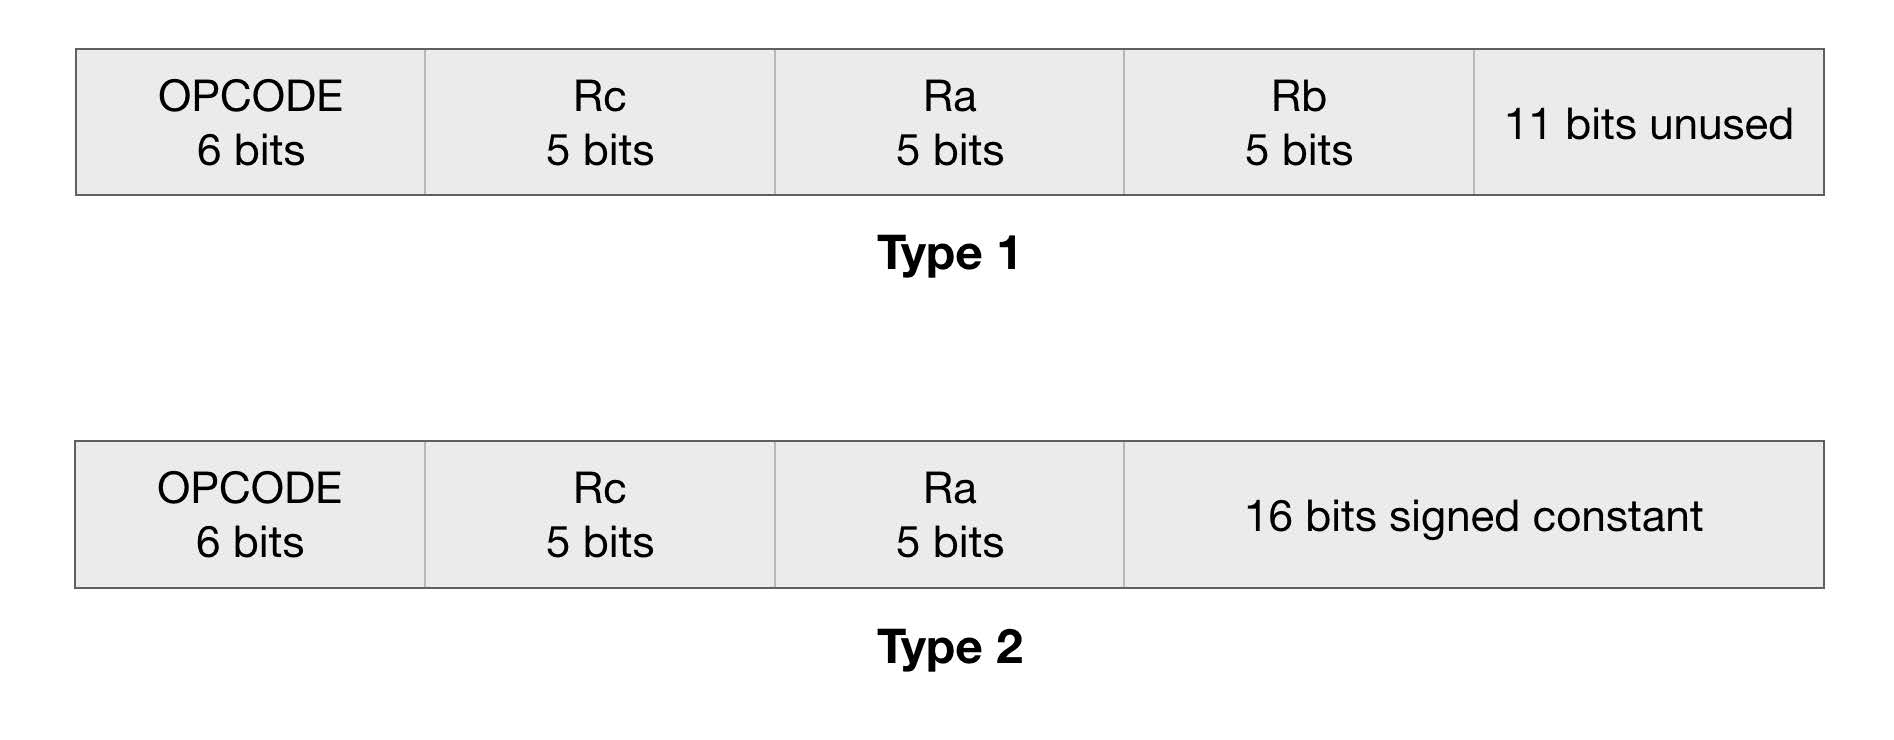
\includegraphics[width = 7cm]{beta_instruction_format}
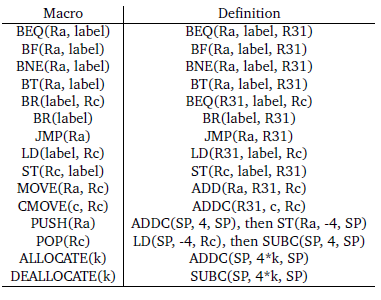
\includegraphics[width = 7cm]{Macro}

\end{multicols*}
\end{document}